\documentclass[UTF8]{ctexart}
\usepackage{geometry, CJKutf8}
\geometry{margin=1.5cm, vmargin={0pt,1cm}}
\setlength{\topmargin}{-1cm}
\setlength{\paperheight}{29.7cm}
\setlength{\textheight}{25.3cm}

% useful packages.
\usepackage{xcolor}
\usepackage{amsfonts}
\usepackage{amsmath}
\usepackage{amssymb}
\usepackage{amsthm}
\usepackage{enumerate}
\usepackage{graphicx}
\usepackage{multicol}
\usepackage{fancyhdr}
\usepackage{layout}
\usepackage{listings}
\usepackage{float, caption}

\lstset{  
  basicstyle=\ttfamily,  
  backgroundcolor=\color{white},  
  frame=single,  
  framesep=5pt,  
  rulecolor=\color{black},   
  breaklines=true,  
  xleftmargin=\parindent,  
  xrightmargin=\parindent  
}  

% some common command
\newcommand{\dif}{\mathrm{d}}
\newcommand{\avg}[1]{\left\langle #1 \right\rangle}
\newcommand{\difFrac}[2]{\frac{\dif #1}{\dif #2}}
\newcommand{\pdfFrac}[2]{\frac{\partial #1}{\partial #2}}
\newcommand{\OFL}{\mathrm{OFL}}
\newcommand{\UFL}{\mathrm{UFL}}
\newcommand{\fl}{\mathrm{fl}}
\newcommand{\op}{\odot}
\newcommand{\Eabs}{E_{\mathrm{abs}}}
\newcommand{\Erel}{E_{\mathrm{rel}}}

\begin{document}

\pagestyle{fancy}
\fancyhead{}
\lhead{骆弘毅, 3210103287}
\chead{数据结构与算法第五次作业}
\rhead{Nov.2nd, 2024}

\section{remove函数的设计思路}
\indent 本次作业要求修改remove函数,以达到避免进行节点复制的操作(由于节点内容不确定,因此无法保证复制的效率)。同时原来的代码最后一步还需要重新做一遍删除,这在树深很大的时候会非常影响效率。因此我们选择了节点替换的方式,即改变指针的指向来调整BST的结构。而相应的,虽然效率上得到了保证(因为可以在常数时间内完成remove),代码会变得较为复杂,这次作业中在删除倒数第二层节点和根节点时都需要单独进行处理,因此在写程序时还是遇到了不少的困难。\\
\indent 在修改后的代码中,我新增了一个函数detachMin,用于寻找根节点下的最小节点,返回该最小节点并删除,此处由于需要将最小节点的右子树链接到最小节点的父母,而在实际编写过程中我发现,如果该节点的子树退化为一个只有右子树的单链表时,最小值就是根节点本身,这种情况下需要把右子树链接到根节点的父母,因此我相对于提示给的参数列表做了些许调整,即加入了一个根节点的父母节点,由于我们默认选择右子树的最小节点,因此不用考虑左子树还是右子树的问题。在这些设定下,整个函数的逻辑就很清晰了,我们传入根节点和其父母,先判断该节点是否为空,或者已经是最小节点,若是,则进行单独处理,若不是,则往左子树一直搜索,并实时记录当前节点的父母节点,找到最小节点后,将右子树链接到其父母并返回该节点即可。\\
\indent 再看到remove函数,找到要删除的节点和之前代码并无区别。remove函数还是分为无孩子,单孩子和双孩子三种情况处理。顺带一提,虽然此处单孩子和无孩子的情况比较简单,对比原先课本的代码,我用choice分别记录了该节点的父母节点和是左子树还是右子树的信息,而课本代码则是巧妙运用了在递归形式下使用左值引用,可以在改变t的地址信息的同时完成其父母的链接(将节点的左子树信息或右子树信息作为左值引用进入函数体,可以巧妙的避免父母信息的记录)。而双孩子的情况,我首先记录了原先节点的左右子树的根节点信息,然后调用detachMin函数返回右子树的最小节点,然后将左右子树接上去。同时由于在找到最小节点的过程中记录了父母节点的信息,我们再将父母节点指向该节点即可。此处比较需要注意的点有两个,一个是整棵树的根节点删除,一个是倒数第二行根节点的删除。第一个点需要注意的原因是最终会改变根节点的地址,第二个点需要注意的原因是替换节点和原先的右子树节点是同一节点,因此如果按照正常连接方式会出现指向自己的情况,因此均需要单独进行处理。

\section{测试设计与分析}
\indent 此处我选用的测试用例是一个三层的完全二叉树,并以此为基础做一些删除操作,最初的形式如下图所示
\begin{figure}[htbp] 
\centering 
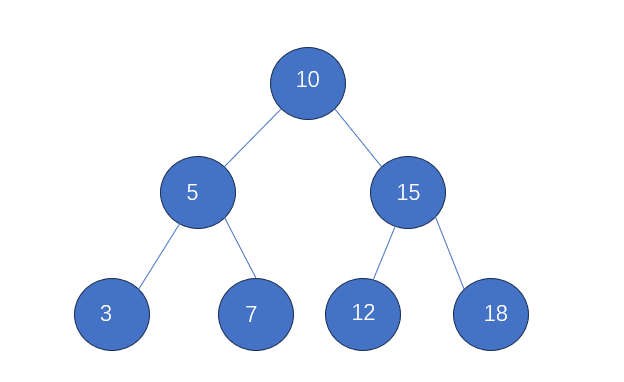
\includegraphics[width=0.5\textwidth]{1.png} 
\caption{二叉树图示}
\end{figure}
\newpage
\noindent 接着对这个二叉树做以下操作:\\
1、删除18并打印\\
2、添加18,删除15,打印\\
3、添加15,删除10,打印\\
虽然看上去删除后又添加回去,实际上第二次添加已经改变了二叉树的结构,这三个测试是分别为了测试叶子节点,倒数第二行的节点,和根节点的删除操作。通过valgrind检验内存泄漏,最终发现无内存泄漏。经检验,结果和预期相符,结果如下:\\
\begin{figure}[!h] 
\centering 
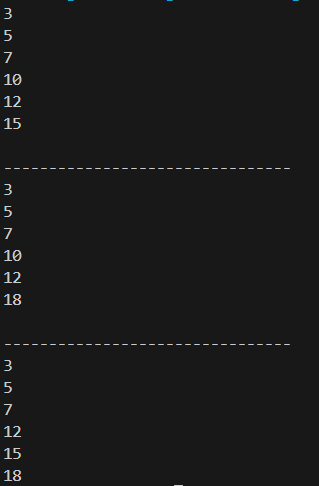
\includegraphics[width=0.5\textwidth]{2.png} 
\caption{输出结果}
\end{figure}
\begin{figure}[!h] 
\centering 
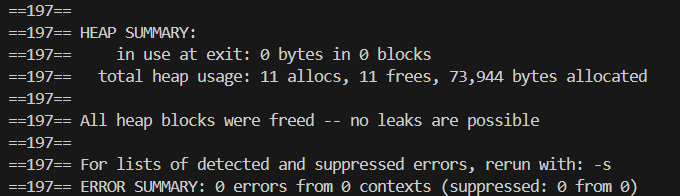
\includegraphics[width=0.5\textwidth]{3.png} 
\caption{内存泄漏检测}
\end{figure}
\end{document}

%%% Local Variables: 
%%% mode: latex
%%% TeX-master: t
%%% End: 
